
\section{La organización en Twitter, Inc.}

La función de organización se basa, principalmente, en dividir el trabajo, tanto humano como material, para posteriormente coordinar las distintas tareas de forma agrupada para la correcta ejecución de los planes establecidos. Para esta organización debemos tener en cuenta distintos factores, como la misión, los objetivos de la empresa, el uso de herramientas para la construcción de esta estructura, entre otros.

Twitter, Inc. mantiene, claramente, una estructura adhocratica, debido a su complejidad y a su dinamismo.

En la empresa que analizamos, Twitter, Inc., ya hemos mencionado anteriormente algunos de estos (como la misión).

\newpage

\subsection{Organigrama.}

\begin{figure}[!htb]
\centering
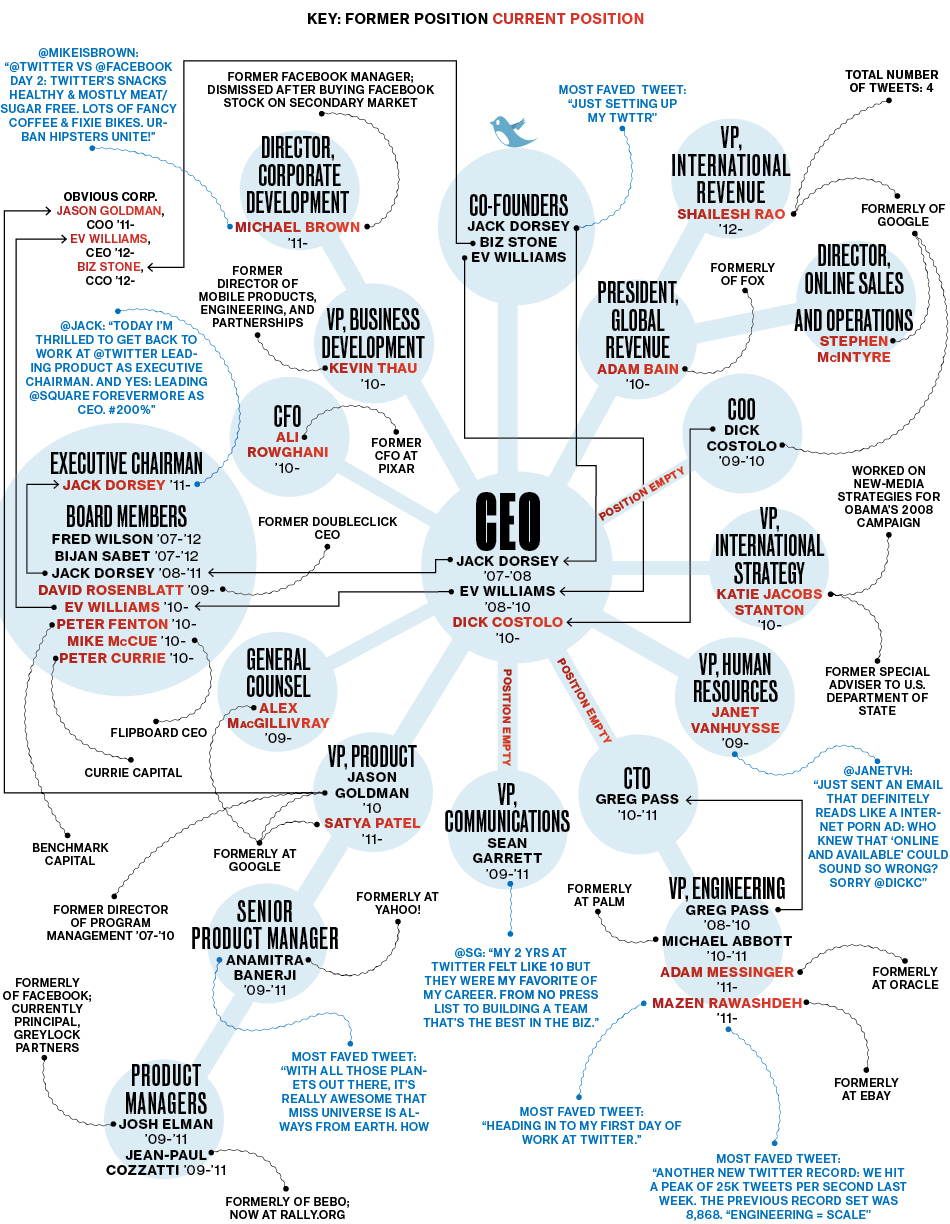
\includegraphics[scale=0.2]{organigrama.jpg}
\caption{\label{fig:frog}Organigrama Twitter, Inc. 2012}
\end{figure}


\subsection{Principios organizativos fundamentales.}

\subsubsection{Principio de la división del trabajo.}

Siguiendo estos principio, Twitter, Inc., se distribuye en distintos equipos de trabajo, entre los que se encuentran:\\

\textbf{Construir el producto}

El grupo \textit{Build the product} comprende los siguientes equipos:

\begin{itemize}

\item \textit{Data Science and Analytics}

Encargado de comprender como el mundo utiliza Twitter y como son sus usuarios.

\item \textit{Infraestructure Engineering}

Encargado de innovar, construir y mantener la infraestructura y servicios de Twitter operativos.

\item \textit{Product}

Encargado de desarrollar el producto principal, Twitter.

\item \textit{Software Engineering}

Encargado de desarrollar todos los servicios necesarios  en los que se basa Twitter, como por ejemplo Bootstrap.

\item \textit{User Services}

Encargado de dar soporte a los usuarios de Twitter siempre que lo necesiten.

\item \textit{Design and Research}

Encargados de mantener el diseño y características de Twitter a la última.

\end{itemize}

\textbf{Grupo: Seguir manteniéndonos}

El grupo \textit{Keep us running} comprende los siguientes equipos:

\begin{itemize}

\item \textit{Finance}

Encargado de controlar las finanzas de Twitter, haciendo posible que sus productos sean rentables.

\item \textit{Legal and Public Policy}

Encargado de defender legalmente a la compañía y a sus usuario. 

\item \textit{People}

Encargado de los Recursos Humanos de Twitter, intentando que sea un lugar serio a la vez que agradable para trabajar.

\item \textit{Workplace}

Encargado de que las oficinas de Twitter sean lo más cómodas y útiles, para un correcto desarrollo de sus empleados.

\end{itemize}

\textbf{Grupo: Promover el negocio}

El grupo \textit{Promote the business} comprende los siguientes equipos:

\begin{itemize}

\item \textit{Marketing and Communications}

Encargado de enseñar al mundo los avances realizados en Twitter.

\item \textit{Sales and Partnerships}

Encargado de trabajar en conjunto con otras marcas y compañías para alcanzar sus objetivos de forma conjunta y más sencilla.

\end{itemize}

\textbf{Grupo: Nuestras marcas}

El grupo \textit{Our family of brands} comprende los siguientes equipos:

\begin{itemize}

\item \textit{Periscope}
\item \textit{MoPub}\\

\end{itemize}



Todos estos equipos se distribuyen entre más 35 países alrededor del mundo.

\subsubsection{Principio de la especialización del trabajo.}

Como vemos en el apartado anterior, existen grandes distinciones entre los distintos equipos de trabajo, por lo que es necesaria una especialización, que dependerá de cada equipo, encontrando así un alto nivel de especialización en cada uno de ellos.

\subsubsection{Principio de jerarquía, unidad de mando y ámbito de control.}

Estos principios, explicados y revisados en apartados anteriores, suponen una correcta organización del trabajo, esencial para el desarrollo de los objetivos de la empresa.

\subsubsection{Principio de descentralización.}

Como hemos visto, en Twitter, Inc. vemos una clara descentralización con los distintos grupos de trabajo, sin obviar las decisiones tomadas por los altos directivos.